\documentclass[11pt,letterpaper]{article}
\PassOptionsToPackage{hyphens}{url}
\usepackage[margin=.83in,top=.8in,bottom=.8in,headheight=15pt]{geometry}
\usepackage[T1]{fontenc}
\usepackage{lmodern,amsmath,amssymb,mathtools,bm,booktabs,array,graphicx,tikz}
\usetikzlibrary{arrows.meta,positioning,calc,decorations.pathreplacing,patterns}
\definecolor{ink}{HTML}{17344D}\definecolor{accent}{HTML}{087E8B}\definecolor{pale}{HTML}{EDF5F5}\definecolor{gold}{HTML}{AD6B19}
\providecommand{\dd}{\,\mathrm{d}}\providecommand{\R}{\mathbb{R}}
\providecommand{\E}{\mathbb{E}}\providecommand{\Var}{\operatorname{Var}}
\providecommand{\Cov}{\operatorname{Cov}}\providecommand{\diag}{\operatorname{diag}}
\providecommand{\norm}[1]{\left\lVert#1\right\rVert}
\providecommand{\abs}[1]{\left|#1\right|}
\usepackage{microtype,hyperref,fancyhdr,enumitem,amsthm,sectsty,needspace}
\allsectionsfont{\raggedright}
\hypersetup{colorlinks=true,linkcolor=ink,urlcolor=accent,pdfauthor={Zan Ahmad},pdftitle={Planar viscous flow and boundary-value discretization / Lecture notes}}
\setlength{\parindent}{0pt}\setlength{\parskip}{6pt}\linespread{1.07}
\setlist{itemsep=3pt,topsep=4pt,leftmargin=*}
\emergencystretch=2em\clubpenalty=10000\widowpenalty=10000
\pagestyle{fancy}\fancyhf{}\fancyhead[L]{\small Computational Cardiology}\fancyhead[R]{\small Lecture 7}
\fancyfoot[L]{\footnotesize Zan Ahmad}\fancyfoot[R]{\footnotesize\thepage}\renewcommand{\headrulewidth}{.3pt}
\newtheorem{proposition}{Proposition}\newtheorem{theorem}{Theorem}\newtheorem{lemma}{Lemma}
\theoremstyle{definition}\newtheorem{definition}{Definition}\newtheorem{example}{Example}
\numberwithin{equation}{section}
\begin{document}
{\small\scshape Computational Cardiology\hfill Lecture 7}\par\medskip
{\raggedright\hyphenpenalty=10000\exhyphenpenalty=10000\LARGE\bfseries\color{ink} Planar viscous flow and boundary-value discretization\par}\medskip
{\small Lecture notes}\par\bigskip
Incompressibility constrains a velocity field but does not determine it. For fully developed planar flow, the momentum equation reduces to a second-order boundary-value problem. Its quadratic solution makes it possible to distinguish exact nodal reconstruction from the error introduced by integrating that reconstruction.

\section{Incompressibility and the missing momentum equation}
\hypertarget{note-incompressibility-and-the-missing-momentum-equation}{}\label{note:incompressibility-and-the-missing-momentum-equation}
{\small \href{slides.html\#frame=the-incompressible-balance\&step=1}{Slides for this section} \quad \href{../modules/cfd/index.html}{Conservation, viscous flow and transport} \quad \href{../modules/animations/conservation-flow.html}{Conservation and channel flow}}\par
An incompressible constant-density fluid conserves volume locally. For a fixed control volume, total outward volume flux must sum to zero when no source is present. Shrinking the control volume gives the zero-divergence condition. This condition restricts how velocity components can vary, but it does not tell us how large the velocity is or which pressure field drives it. A momentum balance and appropriate boundary data are also needed.

A particularly useful benchmark is flow between parallel stationary plates. Let x point downstream and y measure distance from the lower wall. Assume a steady fully developed profile with only the downstream component u(y). Its x derivative is zero and its transverse component is zero, so divergence vanishes identically. Many possible functions of y meet that condition. Incompressibility alone cannot select the familiar parabola.

The geometry and assumptions are part of the problem statement: plate separation H, a long straight channel region away from entrance effects, constant dynamic viscosity \ensuremath{\mu}, no body force in the flow direction, and a prescribed constant pressure gradient. These reductions make a transparent test possible. They also define its limits. Passing this benchmark does not test moving curved walls, inlet development, unsteady inertia or a general pressure--velocity coupling algorithm.

\[
\nabla\!\cdot\mathbf u=0,\qquad \oint_{\partial\Omega}\mathbf u\!\cdot\mathbf n\,dS=0
\]
The integral statement applies to a fixed region with no volume source.

\[
\mathbf u=(u(y),0),\qquad \partial_xu+\partial_yv=0
\]
Momentum and wall conditions still determine which profile is selected.

For $\boldsymbol u=(u(y),0)$, the divergence is zero for every differentiable $u$. The momentum equation supplies the missing constraint. Under the stated steady, fully developed assumptions, $\boldsymbol u\cdot\nabla\boldsymbol u=u(y)\partial_x\boldsymbol u=0$, leaving the pressure gradient balanced by viscous curvature.
\section{Integration of the reduced momentum balance}
\hypertarget{note-integration-of-the-reduced-momentum-balance}{}\label{note:integration-of-the-reduced-momentum-balance}
{\small \href{slides.html\#frame=reduced-momentum\&step=1}{Slides for this section} \quad \href{../modules/cfd/index.html}{Conservation, viscous flow and transport} \quad \href{../modules/animations/conservation-flow.html}{Conservation and channel flow}}\par
Under the stated assumptions, the downstream momentum equation balances the pressure gradient with viscous curvature. Write G=\ensuremath{-}dp/dx, so positive G drives positive downstream flow. The reduced equation is \ensuremath{\mu}u\ensuremath{^{\prime\prime}}=\ensuremath{-}G. Integrating twice gives a quadratic plus two constants. The constants are determined by the two wall velocities, not by incompressibility or a preferred plotting convention.

For stationary no-slip plates, u(0)=u(H)=0. The lower condition eliminates the constant offset. The upper condition fixes the linear term, leaving G y(H\ensuremath{-}y)/(2\ensuremath{\mu}). The maximum occurs halfway across the gap and equals GH\ensuremath{^{2}}/(8\ensuremath{\mu}). Integrating across the gap gives flow per out-of-plane width q=GH\ensuremath{^{3}}/(12\ensuremath{\mu}). Its units are square meters per second. Multiply by the channel width W to obtain a volume rate in cubic meters per second.

A unit check helps catch a common confusion with hydraulic resistance. G has pressure per length, while \ensuremath{\mu} has pressure times time. Their ratio has inverse length per time; multiplication by y(H\ensuremath{-}y) gives length per time, the required speed unit. The pressure drop across a channel length L is GL. Reversing the pressure gradient reverses the entire velocity and flux, while doubling viscosity halves them at fixed G and geometry.

\[
\mu u^{\prime\prime}=-G,\quad G=-dp/dx,\quad u(0)=u(H)=0
\]
\ensuremath{\mu} is Pa\ensuremath{\cdot}s; G is Pa/m.

\[
u(y)=\frac{G}{2\mu}y(H-y),\quad u_{\max}=\frac{GH^2}{8\mu},\quad q=\frac{GH^3}{12\mu},\quad Q=Wq
\]
H and W are in meters; u is m/s, q is m\ensuremath{^{2}}/s and Q is m\ensuremath{^{3}}/s.

With wall velocities $U_0$ and $U_H$, two integrations give
\[
 u(y)=\frac{G}{2\mu}y(H-y)+U_0+\frac{U_H-U_0}{H}y.
\]
The last two terms are the unique linear function satisfying the wall data. The corresponding flow per width is
\[
 q=\frac{GH^3}{12\mu}+\frac H2(U_0+U_H).
\]
Superposition is possible because the reduced equation and boundary conditions are linear.
\section{Pressure-driven and moving-wall flow}
\hypertarget{note-pressure-driven-and-moving-wall-flow}{}\label{note:pressure-driven-and-moving-wall-flow}
{\small \href{slides.html\#frame=flux-and-maximum-speed\&step=1}{Slides for this section} \quad \href{../modules/cfd/index.html}{Conservation, viscous flow and transport} \quad \href{../modules/animations/conservation-flow.html}{Conservation and channel flow}}\par
Use H=0.002 m, \ensuremath{\mu}=0.004 Pa\ensuremath{\cdot}s and G=100 Pa/m. The center speed is 0.0125 m/s, or 12.5 mm/s. The cross-sectional mean speed is two-thirds of that, approximately 0.008333 m/s. Flow per width is 1.6667\ensuremath{\times}10\ensuremath{^{-5}} m\ensuremath{^{2}}/s. With W=0.01 m, total flow is 1.6667\ensuremath{\times}10\ensuremath{^{-7}} m\ensuremath{^{3}}/s, or approximately 0.166667 mL/s. These are transparent teaching parameters rather than a claim about a particular vessel.

For a 0.1 m channel segment the pressure drop would be 10 Pa. Using density 1060 kg/m\ensuremath{^{3}} and the gap H as the characteristic length gives a Reynolds number of approximately 4.42. State the chosen length convention: a hydraulic-diameter convention would yield another numeric value. This ratio describes inertia relative to viscosity on the specified scales. It does not by itself prove that all fully developed assumptions apply at a physical inlet.

Now move only the upper wall at 0.02 m/s while keeping the lower wall stationary and G fixed. A linear contribution of 0.02 y/H is added to the pressure-driven parabola. The center speed becomes 0.0225 m/s and flow per width increases by H times half the wall speed, or 2\ensuremath{\times}10\ensuremath{^{-5}} m\ensuremath{^{2}}/s. This controlled boundary change illustrates why a verified interior equation can produce the wrong physical result when its boundary values are wrong.

For stationary walls, pressure drop $\Delta p=GL$ gives the hydraulic resistance
\[
 R_{\rm channel}=\frac{\Delta p}{Q}=\frac{12\mu L}{WH^3}.
\]
The cubic dependence on gap is a consequence of this planar geometry. It is distinct from the fourth-power radius law for a circular tube. The center-to-mean velocity ratio is $u_{\max}/\overline u=3/2$.

\paragraph{Calculation.} Calculate center speed, mean speed and total flow for the stationary-wall benchmark.

Use GH\ensuremath{^{2}}/(8\ensuremath{\mu})=100\ensuremath{\times}0.002\ensuremath{^{2}}/(8\ensuremath{\times}0.004)=0.0125 m/s.

Use q=GH\ensuremath{^{3}}/(12\ensuremath{\mu})=1.6667\ensuremath{\times}10\ensuremath{^{-5}} m\ensuremath{^{2}}/s, so q/H=0.008333 m/s.

Multiply q by 0.01 m width and by 10\ensuremath{^{6}} mL/m\ensuremath{^{3}} to obtain 0.166667 mL/s.

All three quantities have distinct definitions and compatible units.
\begin{center}\begin{minipage}{.98\linewidth}\centering
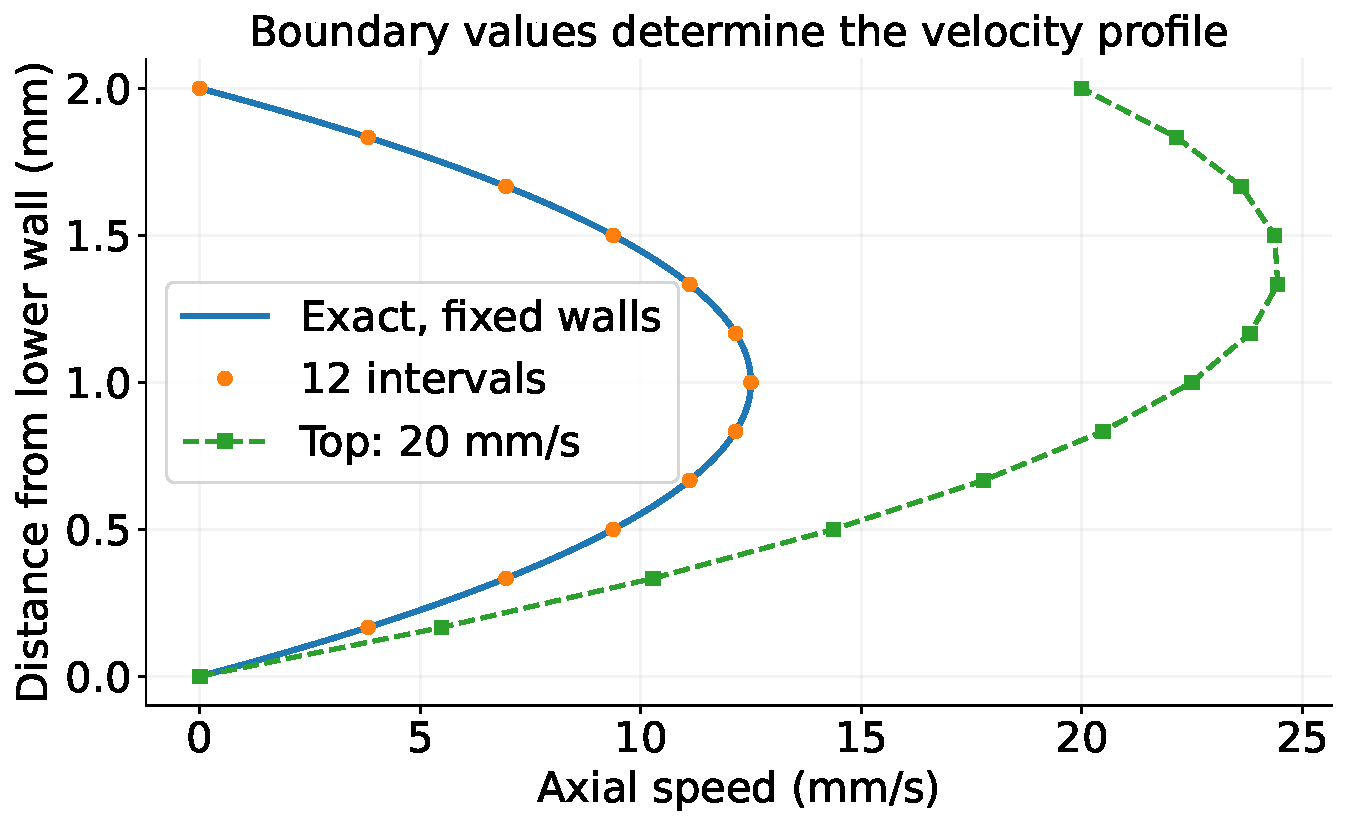
\includegraphics[width=.96\linewidth,height=.57\textheight,keepaspectratio]{channel-profiles.pdf}\par\smallskip
{\small Original reduced channel calculation: H=\allowbreak{}2 mm, $\mu$=\allowbreak{}0.004 Pa$\cdot$s and G=\allowbreak{}100 Pa/m. Moving the upper wall adds a linear component.}
\end{minipage}\end{center}
\section{The discrete Dirichlet problem}
\hypertarget{note-the-discrete-dirichlet-problem}{}\label{note:the-discrete-dirichlet-problem}
{\small \href{slides.html\#frame=centered-interior-equations\&step=1}{Slides for this section} \quad \href{../modules/cfd/index.html}{Conservation, viscous flow and transport}}\par
Divide the gap into N equal intervals and store velocity at N+1 nodes, including both walls. At each interior node, approximate the second derivative by the centered second difference. After multiplying by spacing squared and arranging signs, the matrix has two on the diagonal and minus one on the neighboring diagonals. The right side is Gh\ensuremath{^{2}}/\ensuremath{\mu}, with the known wall velocities added at the first and last interior rows.

The unknowns are all interior velocities solved simultaneously. This is a steady boundary-value solve; there is no time step or CFL restriction in this code. Positive viscosity and a positive gap make the stated problem well posed. The implementation uses a banded linear solver, checks finite inputs and outputs, and reports the algebraic residual. A small algebraic residual means the discrete equations were solved closely, not that every continuous or physical error has vanished.

This benchmark contains a useful trap: the centered second difference is exact for a quadratic at the nodes. With exact boundary values, our particular nodal scheme reproduces the analytic parabola to roundoff. Its nodal error therefore cannot reveal an ordinary second-order refinement slope. The DOE MFiX benchmark uses its own discretization and reports its own convergence behavior; we do not transfer that observed result to our different implementation.

\[
2u_j-u_{j-1}-u_{j+1}=Gh^2/\mu,\qquad h=H/N
\]
Known wall values move to the right side of the first and last interior equations.

Let $A$ be the tridiagonal matrix with diagonal $2$ and off-diagonal $-1$. For a vector with homogeneous endpoint values,
\[
 z^{\mathsf T}Az=\sum_{j=0}^{N-1}(z_{j+1}-z_j)^2>0
\]
unless every value vanishes. Thus the discrete Dirichlet problem has a unique solution. Nonzero wall values enter the first and last right-hand-side entries; changing them changes the solution without changing the interior operator.
\section{Exact nodal values and inexact quadrature}
\hypertarget{note-exact-nodal-values-and-inexact-quadrature}{}\label{note:exact-nodal-values-and-inexact-quadrature}
{\small \href{slides.html\#frame=exact-differentiation-of-a-quadratic\&step=1}{Slides for this section} \quad \href{../modules/cfd/index.html}{Conservation, viscous flow and transport}}\par
To report total flow from the computed nodal profile, the demo applies the composite trapezoidal rule. Straight line segments connecting a concave parabola lie below the curve, so this integral underestimates the true flow even when every node is exact. The profile solve and the integral approximation are separate numerical operations. They deserve separate diagnostics and separate labels in a convergence plot.

For the stationary-wall quadratic on N equal intervals, the trapezoidal flow is exactly q times (1\ensuremath{-}1/N\ensuremath{^{2}}) in real arithmetic. The relative error is therefore 1/N\ensuremath{^{2}}. At N=4 it is 6.25 percent, at N=8 it is 1.5625 percent, and at N=16 it is 0.390625 percent. Halving spacing divides this error by four. The plotted order of two describes integration of the profile, not a measured nodal-profile discretization order.

A linear Couette contribution is integrated exactly by the trapezoidal rule, so the absolute error associated with the pressure-driven quadratic remains the same at fixed G, H and N. The relative error in the combined flow can change because the denominator changes. State whether an error is absolute or relative before comparing cases.

\[
q_h=h\left(\frac{u_0+u_N}{2}+\sum_{j=1}^{N-1}u_j\right),\qquad \frac{q-q_h}{q}=\frac1{N^2}
\]
The relative-error expression assumes nonzero pressure-driven flow with stationary walls.

For $u(y)=a y(H-y)$, the exact integral is $aH^3/6$. Using $\sum_{j=1}^{N-1}j=N(N-1)/2$ and $\sum_{j=1}^{N-1}j^2=N(N-1)(2N-1)/6$ in the trapezoidal sum gives
\[
 q_h=\frac{aH^3}{6}\left(1-\frac1{N^2}\right).
\]
A linear Couette contribution is integrated exactly, so it changes the denominator of a relative error but not the absolute pressure-driven quadrature error.
\begin{center}\begin{minipage}{.98\linewidth}\centering
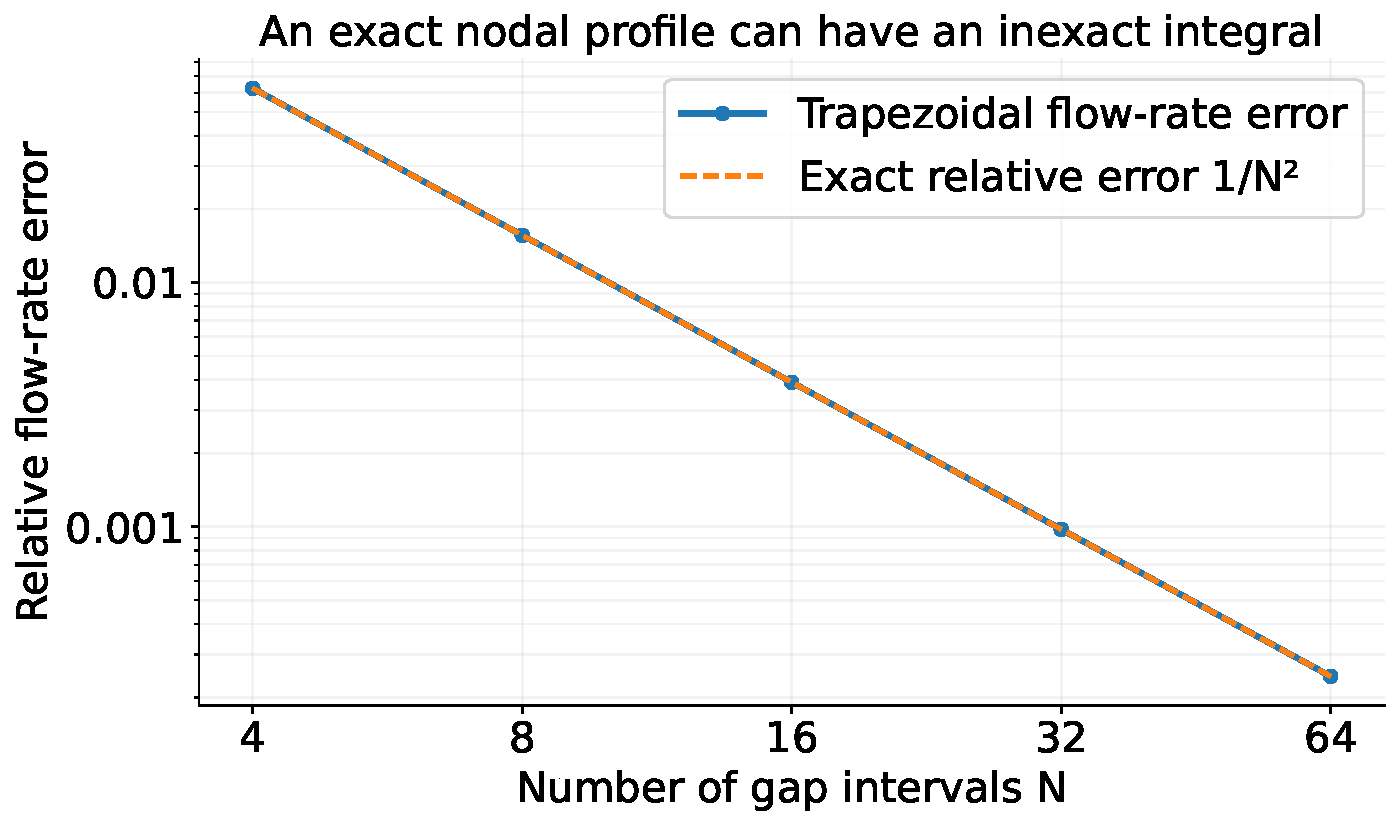
\includegraphics[width=.96\linewidth,height=.57\textheight,keepaspectratio]{channel-flux-error.pdf}\par\smallskip
{\small The exact nodal quadratic is integrated by trapezoids. Relative flow error follows 1/N$^2$; this is not a profile-error convergence claim.}
\end{minipage}\end{center}
\section{Linearity, boundary data and physical scope}
\hypertarget{note-linearity-boundary-data-and-physical-scope}{}\label{note:linearity-boundary-data-and-physical-scope}
{\small \href{slides.html\#frame=changing-the-wall-velocity\&step=1}{Slides for this section} \quad \href{../modules/cfd/index.html}{Conservation, viscous flow and transport}}\par
The author checks include a zero-gradient stationary fluid, reversal of the pressure gradient, doubling the gradient, and pure moving-wall flow with zero gradient. These limiting cases exercise signs, linearity and the insertion of boundary values. A profile comparison tests the analytic solution, while an algebraic residual tests the linear solve and a quadrature comparison tests the reported integral. None substitutes for the others.

The reduced solution contains no entrance region or developing transverse velocity. A Reynolds number formed with gap $H$ is $\mathrm{Re}=\rho\overline uH/\mu$; using another characteristic length changes its numerical value. The fully developed ansatz, wall conditions and selected geometry remain assumptions even when the reduced boundary-value problem is solved exactly.
\bigskip
\section*{Exercises}
\par\noindent\begin{minipage}{\linewidth}
\subsection*{E1. Pressure-driven flow with units}
Use H=\allowbreak{}0.003 m, $\mu$=\allowbreak{}0.003 Pa$\cdot$s, G=\allowbreak{}80 Pa/m and W=\allowbreak{}0.012 m.

\textbf{a} Calculate the center speed and mean speed.

\end{minipage}\par\medskip
\textbf{b} Calculate flow per width and total flow in mL/s.

\textbf{c} If the pressure drop is 4 Pa, what segment length is consistent with G?

\par\noindent\begin{minipage}{\linewidth}
\subsection*{E2. Boundary values matter}
For the lesson benchmark H=\allowbreak{}0.002 m, $\mu$=\allowbreak{}0.004 Pa$\cdot$s and G=\allowbreak{}100 Pa/m, move the upper wall at 0.01 m/s and keep the lower wall fixed.

\textbf{a} Write the full profile and evaluate it at the center.

\end{minipage}\par\medskip
\textbf{b} Compute the added flow per width.

\textbf{c} Would a code that silently keeps the upper wall stationary pass the original stationary-wall benchmark? Explain.

\par\noindent\begin{minipage}{\linewidth}
\subsection*{E3. Exact nodes and an imperfect flow rate}
A stationary-wall channel has exact flow per width q=\allowbreak{}2$\times$10$^-$$^5$ m$^2$/s. Its nodal quadratic is integrated by trapezoids.

\textbf{a} Calculate q\_h and relative error for N=\allowbreak{}5 and N=\allowbreak{}10 intervals.

\end{minipage}\par\medskip
\textbf{b} Identify the observed order and the numerical operation it measures.

\textbf{c} Explain why dividing by q is inappropriate at G=\allowbreak{}0 with stationary walls.

\par\noindent\begin{minipage}{\linewidth}
\subsection*{E4. What does incompressibility leave undetermined?}
Consider u(y)=\allowbreak{}U sin($\pi$y/H), v=\allowbreak{}0 in a straight channel, with U>0 and no x dependence.

\textbf{a} Does this field satisfy divergence-free flow and stationary no-slip walls?

\end{minipage}\par\medskip
\textbf{b} Does it satisfy the constant-gradient Poiseuille momentum equation?

\section*{References}
\noindent\begin{minipage}{\linewidth}
Zan Ahmad, Advanced Topics in Computational Cardiology syllabus, Fall 2024. PDF pages 1--2.

\end{minipage}\par\medskip
\noindent\begin{minipage}{\linewidth}
DOE NETL MFiX, FLD01: Steady, 2D Poiseuille flow. Sections 3.1.1 and 3.1.3; equations 3.1--3.2.

\url{https://mfix.netl.doe.gov/doc/vvuq-manual/main/html/fluid/fld-01.html}
\end{minipage}\par\medskip
\end{document}
